\documentclass[../Cours.tex]{subfiles}

\usepackage{xstring}
\usepackage{xfp}

\begin{document}
\clearpage
\thispagestyle{empty}

\titreDScorrection

\begin{questions}
    \EXERCICETITRE{4}{DISTANCE D'ARRÊT}
    \question Si une voiture roule à \qty{20}{\metre\per\second}, cela signifie qu'elle parcourt \qty{20}{\metre} en 1 seconde. Or, la distance de réaction est d'une seconde, donc la distance de réaction est de \qty{20}{\metre}.

    \question On va ici utiliser la formule donnée juste avant la question : 
        $$D_f = \dfrac{v^2}{2 \times g \times a} = \dfrac{20^2}{2 \times 10 \times \num{0.6}} = \qty{33.33}{\metre}$$
        On choisit $a = \num{0.6}$ car il est précisé dans la question que la route est mouillée.
        Donc la distance de freinage est de \qty{33.33}{\metre}.
        
    \question Dans l'énoncé, on dit que << la distance d’arrêt est la somme de la distance de réaction et de la distance de freinage>>. Donc, on va additionner les réponses des deux questions précédentes.

    $$20 + \num{33.33} = \qty{53.33}{\metre}$$
    La distance d'arrêt est donc de \qty{53.33}{\metre}.

    \EXERCICETITRE{4}{Dame blanche}

    \question Ici, on applique la formule du volume d'une boule :
    $$V_{\mbox{boule}} = \frac{4}{3} \times \pi \times \mbox{rayon}^3$$
    On remplace le rayon par la valeur de l'énoncé : \qty{5}{\centi\metre}.
    \begin{align*}
        V_{\mbox{boule}} &= \frac{4}{3} \times \pi \times (\qty{5}{\centi\metre})^3 \\
        &= \frac{4}{3} \times \pi \times (5 \times 5 \times 5) \\
        &= \qty{523.6}{\centi\metre\cubed}
    \end{align*}

    Donc une boule de glace a pour volume \qty{523.5}{\centi\metre\cubed}.

    \question Dans une dame blanche, il y a 3 boules : 2 à la vanille et 1 au chocolat.\\ Donc le volume total de glace nécessaire est de $523{,}6 \times 3 \approx \qty{1571}{\centi\metre\cubed}$. \\ Pour convertir en \unit{\litre}, on sait que $\qty{1}{\litre} = \qty{1000}{\centi\metre\cubed}$, donc $\qty{1571}{\centi\metre\cubed} = \qty{1.571}{\litre}$.

    \EXERCICETITRE{6}{Comparaison des émissions de $CO_2$}

    \question Il est écrit dans l'énoncé que : 
        \begin{itemize}
            \item En France, pour \qty{1}{\kilo\watt\hour} on émet \qty{78}{\gram} de $CO_2$.
            \item En Allemagne, pour \qty{1}{\kilo\watt\hour} on émet \qty{463}{\gram} de $CO_2$.
        \end{itemize}
        Donc l'Allemagne pollue  $\frac{463}{78} \approx \num{5.936} \approx 6$ fois plus que la France.
        
    \question On fait un tableau de proportionnalité : 
        \begin{center}
            \begin{tabularx}{0.6\linewidth}{|C|C|C|}\hline
                Électricité (en kilowattheures) & 1 & ? \\\hline
                Émission de $CO_2$ (en grammes) & 78 & \textcolor{rouge}{\num{1000000}} \\\hline
            \end{tabularx}
        \end{center}
        En faisant un produit en croix, on obtient le calcul : $\dfrac{1 \times \num{1000000}}{78} \approx \qty{12820}{\kilo\watt\hour}$.

    \question On fait un tableau de proportionnalité : 
        \begin{center}
            \begin{tabularx}{0.6\linewidth}{|C|C|C|}\hline
                Électricité (en kilowattheures) & 1 & \textcolor{rouge}{\num{2500}} \\\hline
                Émission de $CO_2$ (en grammes) & 78 & ?  \\\hline
            \end{tabularx}
        \end{center}
        En faisant un produit en croix, on obtient le calcul : $\dfrac{\num{2500} \times 78}{1} = \qty{195000}{\gram}$.

    \EXERCICETITRE{4}{Composition de l'air}
    
    \question On utilise la formule du volume d'un pavé droit vu en cours : 
    \begin{align*}
        V_{\mbox{pavé droit}} &= \mbox{longueur} \times \mbox{largeur} \times \mbox{hauteur} \\
        &= \qty{7}{\metre} \times \qty{5}{\metre} \times \qty{3}{\metre} \\
        &= 7 \times 5 \times 3 \unit{\metre\cubed} \\
        &= \qty{105}{\metre\cubed}
    \end{align*}
    Donc le volume de la salle de classe est de \qty{105}{\metre\cubed}.

    \question Le diazote et le dioxygène sont répartis dans l'air dans le ratio 4:1, pour un total de volume d'air de \qty{105}{\metre\cubed}.

    \begin{center}
        \begin{tabularx}{0.7\linewidth}{|l|C|C|C|}\hline
            & Diazote & Dioxygène & TOTAL \\\hline
            Volume (en mètre cube) & ? & ? & 105 \\\hline
            Ratio & 4 & 1 & 5 \\\hline
        \end{tabularx}
    \end{center}

    En faisant deux produits en croix : 
    \begin{itemize}
        \item Pour le diazote, on trouve $\dfrac{105 \times 4}{5} = \qty{84}{\metre\cubed}$.
        \item Pour le dioxygène, on trouve $\dfrac{105 \times 1}{5} = \qty{21}{\metre\cubed}$.
    \end{itemize}

    \EXERCICETITRE{4}{Symétries}

    \begin{center}
        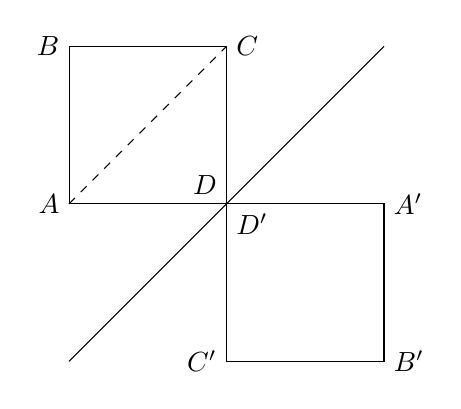
\begin{tikzpicture}
            \draw (0,0) rectangle (2,2);
            \draw[dashed] (0,0) -- (2,2);
            \draw (0,-2) -- (4,2);
            \node[left] at (0,0) {$A$};
            \node[above left] at (2,0) {$D$};
            \node[left] at (0,2) {$B$};
            \node[right] at (2,2) {$C$};
            \draw (2,0) rectangle (4,-2);
            \node[right] at (4,0) {$A'$};
            \node[below right] at (2,0) {$D'$};
            \node[right] at (4,-2) {$B'$};
            \node[left] at (2,-2) {$C'$};
        \end{tikzpicture}
    \end{center}

    \EXERCICETITRE{2}{Une grande multiplication}

    \question On veut connaître le chiffre des unités de $1 \times 3 \times 5 \times ... \times 2017$. On remarque que tous les nombres sont impairs, donc le résultat est aussi impair, ce qui signifie que son chiffre des unités est soit 1, 3, 5, 7 ou 9.\\
    
    Ensuite, puisque dans la multiplication il y a le nombre 5, cela signifie que la réponse est un multiple de 5. Donc son chiffre des unités est soit 5 soit 0.\\
    
    En combinant les deux conditions expliquées ci-dessus, la seule possibilité commune est que le chiffre des unités soit le 5.\\

    Pour information, $1 \times 3 \times 5 \times ... \times 2017 = \seqsplit{4100314615650397395138723015995530374702513317730804551193971138004928593683185400250640226631295635367335619166049726005004840776745677165885304196363252821036344461989116195324139682985251622107072272948170811891524074699319365750289927178167722800856529451021321661190038557203353829838389827684213668946686089225097390904864235723184234473322492751242904180515038319223611073967165357217253458558967884657999016527963609925287684206790408402068363760949597405783835322219035655627252849042470058539089029997272657943141248907489020039113048063970709271018913551463343327333342365093256183621302175552545531974271766274627396380905567820790145215507162488033612277484414564463822070451750854250005866646406961103924291130286650803399601681144726122547523039793664523602546375870643800289357529969188282772892964110476903020664656659602910895044252041184695282539560721429513102159237171113241342253219616701174977915719040782541844445741139666155103626890840040581681087956193217949773197728014426064368153990142099309522807759538386148807385721646567502293848391185149309595189128685913359553835694956939485827215116403999429124834169170104774751822756691445462250471233063533371956966653898053666796522050358655496008084411297759794878691448362549793792954112402627577664271315963788506981820470308009116897006663375382235358521103353787770293705256708319159725828540033689614744149767774765995155940829616338635231976478040387165522130891152624525174667368265141812247279630891059774502203347367992198683179034235136174449347235613189822088439512616804395832504913741918483473809492795145377789352717801940155063646404008702545123108460499469899174368886641591759888051880963169576916343560880191843220878525454264140376492425457356480483727958825594528306921673943751449848930528307564904243992822595305845495334154299034570747867694989463040588692497264731540090735122128023302683023663305356125608974703990729301454391909881964587898896115770803099730977148221043142005725936403896733696351319282396803051097630345493954784948189966576412226214949805483684594346252778297429384735562053700418029459696234322406456797172803487483263887308515280721283688055253404314950203040510980697118603557614956635094879364061502023211607942972407702643364894218345392731049669585312597695469100484552214463922851223063144777903535830653780848025812742607275893162736390926854718588660907252364453401200766843682170461014149205714808218708872332967828894231970000475889085899137130585316682337667503834805503506197967485774765712737120544127637049863461294894240514303972758370357172942048579441259465934674199519339132223740595570795447526482686852538423746581715132666098375852654243038380401155764769384138514177032888090776566286573266150390110539429081266802633504395360577125975221018735862570781710089561847195547752411245734478302613872839848515424647588251128027536651643458753824234008789062}\textcolor{rouge}{5}$
    
    
\end{questions}
\end{document}